\chapter{Configuración de PiBotJ}
\label{cap:capitulo9}

\begin{flushright}
\begin{minipage}[]{10cm}
\emph{Las ideas no duran mucho. Hay que hacer algo con ellas}\\
\end{minipage}\\

Santiago Ramón y Cajal\\
\end{flushright}

\vspace{1cm}

\setcounter{footnote}{136} % Establecer la numeración de la siguiente nota al pie
Una vez el robot ya está construido, es necesario configurarlo tanto para simulación como para poder ejecutarlo en la vida real. Para ello, es necesario seguir los siguientes pasos: 

\section{Simulación}
\label{subsec:anexosimulacion}

Primero de todo, hay que instalar los siguientes programas: 

\begin{verbatim}
	sudo apt update && sudo apt upgrade
	sudo apt install ros-humble-ros2-control ros-humble-ros2-controllers
	sudo apt install ros-humble-rviz2
	sudo apt install ros-humble-gazebo-ros-pkgs
	sudo apt install ros-humble-xacro ros-humble-robot-state-publisher 
	sudo apt install ros-humble-joint-state-publisher
\end{verbatim}
 
Una vez instalados, únicamente hay que ejecutar el programa que permita que el robot en simulación se inicialice. Para ello, únicamente hay que escribir los siguientes comandos:
\begin{verbatim}
	colcon build --packages-select pibotj_r2c   # compila los paquetes
	source ./install/setup.bash                 # configura variables 
	ros2 launch pibotj_r2c launch_sim.launch.py
\end{verbatim} 

Si la primera vez que se lance el robot ocurre algún error, puede ser normal; se vuelve a repetir el proceso de nuevo.

\section{Robot real}
\label{subsec:anexoconfig}

Hay que seguir los siguientes pasos: 

\begin{enumerate}
	\item Instalar \textit{Raspberry Pi Imager}: \verb|sudo apt install rpi-imager|.
	\item Descargar la imagen de Ubuntu 20.04 Server\footnote{\url{https://releases.ubuntu.com/20.04.6/}}.
	\item Abrir \textit{rpi-imager} y seguir los pasos que aparecen por pantalla.
	\item Conectarse al robot usando \verb|ssh usuario@ip_dispositivo| con la contraseña introducida en el Paso 3.
	\item Una vez conectado con el robot, ya se puede operar con él.
	\item Instalar ROS 2 Foxy\footnote{\url{https://docs.ros.org/en/foxy/Installation/Ubuntu-Install-Debians.html}}.
	\item Configurar cada uno de los componentes del robot.
\end{enumerate}

Al no tener disponible interfaz gráfica, la única forma de comunicarse con el robot es a través de SSH y variantes de esta, como SCP, para copiar directorios entre el robot y el ordenador local.

Otra opción para poder desarrollar código es usar un \textit{plugin} de VSCode (desde el ordenador local) que permite usar VSCode conectándose al robot usando SSH\footnote{\url{https://code.visualstudio.com/docs/remote/ssh-tutorial}}.

\subsection{Cámara}
\label{subsec:anexocamara}

La cámara está conectada al puerto CSI y, para hacerla funcionar, se necesitan  instalar los siguientes programas: 

\begin{verbatim}
	sudo apt-get install gstreamer1.0-tools \ 
	gstreamer1.0-plugins-base gstreamer1.0-plugins-good \ 
	gstreamer1.0-plugins-bad gstreamer1.0-plugins-ugly
\end{verbatim}

Una vez instalados, hay que seguir los siguientes pasos: 

\begin{enumerate}
	\item Editar el fichero \verb|/boot/firmware/config.txt| añadiendo \verb|start_x=1| al final.
	\item Reiniciar la Raspberry: \verb|sudo reboot|.
	\item Comprobar que la configuración es correcta: \verb|v4l2-ctl --list-devices|.
\end{enumerate}\

En la Figura \ref{fig:v4l2} se puede ver el resultado del Paso 3 y muestra que la cámara se encontraba conectada en el dispositivo \verb|/dev/video0|.

\begin{figure} [h!]
	\begin{center}
		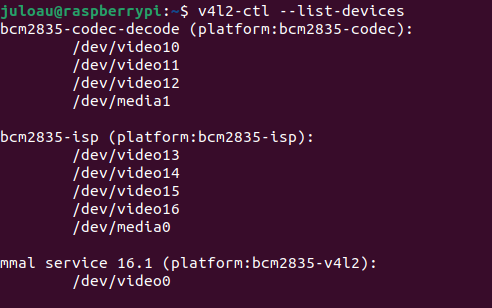
\includegraphics[width=9cm]{figs/cap6/vl.png}
	\end{center}
	\caption{Dispositivos de vídeo y media disponibles en PiBotJ}
	\label{fig:v4l2}
\end{figure}


\subsection{Google Coral}
\label{subsec:anexogooglecoral}


Para su configuración hay que seguir los siguientes pasos: 

\begin{enumerate}
	\item 
	\begin{lstlisting}[language=bash]
		echo "deb https://packages.cloud.google.com/apt \
		coral-edgetpu-stable main" | \
		sudo tee /etc/apt/sources.list.d/coral-edgetpu.list
	\end{lstlisting}

	\item
	\begin{lstlisting}[language=bash]
		curl https://packages.cloud.google.com/apt/doc/apt-key.gpg \
		| sudo apt-key add -
	\end{lstlisting}
	\item \verb|sudo apt-get update|.
	\item \verb|sudo apt-get install libedgetpu1-std|.
	\item Conectar el USB en uno de los puertos 3.0.
	\item \verb|sudo apt-get install python3-pycoral|.
\end{enumerate}\

Finalmente, el proceso se debería haber completado de forma exitosa cuando la salida del último comando se debería ver como muestra la Figura \ref{fig:outcoral}.

\begin{figure} [h!]
	\begin{center}
		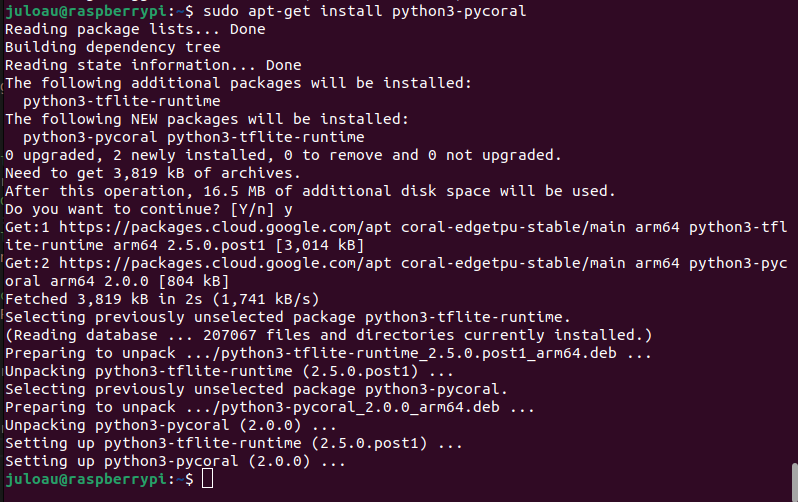
\includegraphics[width=12cm]{figs/cap6/pycoralinstalled.png}
	\end{center}
	\caption{Configuración exitosa del Google Coral}
	\label{fig:outcoral}
\end{figure} 


\subsection{Módulo GPS}
\label{subsec:anexogps}

Hay que seguir los siguientes pasos: 

\begin{enumerate}
	\item Crear el fichero \verb|/etc/udev/rules.d/99-ttyAMA0.rules|.
	\item Añadir: \verb|KERNEL=="ttyAMA0", MODE="0666", GROUP="dialout"|.
	\item \verb|sudo udevadm control --reload-rules|.
	\item \verb|sudo udevadm trigger|.
	\item Las reglas se habrán actualizado. 
	\item Instalar \verb|raspi-config|\footnote{\url{https://github.com/EmilGus/install_raspi-config/tree/master}}.
	\item Ejecutar \verb|raspi-config| usando \verb|sudo raspi-config|
	\item Dentro de \textit{raspi-config} hay que desplazarse hasta \textit{Interfacing options} y \textit{serial}.
	\item Deshabilitar \textit{serial login shell} y habilitar \textit{serial interface}.
	\item Reiniciar la Raspberry: \verb|sudo reboot|
\end{enumerate}\

Finalmente, los siguientes ficheros tienen que contener la siguiente información: 

\begin{lstlisting}[language=bash]
	cat /boot/firmware/config.txt 
	
	# Please DO NOT modify this file; if you need to modify the boot config,
	# the "usercfg.txt" file is the place to include user changes. Please 
	# refer to the README file for a description of the various configuration 
	# files on the boot partition.
	
	# The unusual ordering below is deliberate; older firmwares (in particular 
	# the version initially shipped with bionic) don't understand the conditional
	# [sections] below and simply ignore them. The Pi4 doesn't boot at all 
	# with firmwares this old so it's safe to place at the top. Of the Pi2 and 
	# Pi3, the Pi3 uboot happens to work happily on the Pi2, so it needs to go 
	# at the bottom to support old firmwares.
	
	[pi4]
	kernel=uboot_rpi_4.bin
	
	[pi2]
	kernel=uboot_rpi_2.bin
	
	[pi3]
	kernel=uboot_rpi_3.bin
	
	[pi0]
	kernel=uboot_rpi_3.bin
	
	[all]
	device_tree_address=0x03000000
	
	[pi4]
	max_framebuffers=2
	arm_boost=1
	
	[all]
	# Enable the audio output, I2C and SPI interfaces on the GPIO header. As these
	# parameters related to the base device-tree they must appear *before* any
	# other dtoverlay= specification
	dtparam=audio=on
	dtparam=i2c_arm=on
	dtparam=spi=on
	
	# Comment out the following line if the edges of the desktop appear outside
	# the edges of your display
	disable_overscan=1
	
	# If you have issues with audio, you may try uncommenting the following line
	# which forces the HDMI output into HDMI mode instead of DVI (which doesn't
	# support audio output)
	#hdmi_drive=2
	
	# Config settings specific to arm64
	arm_64bit=1
	dtoverlay=dwc2
	
	[cm4]
	# Enable the USB2 outputs on the IO board (assuming your CM4 is plugged into
	# such a board)
	dtoverlay=dwc2,dr_mode=host
	
	[all]
	
	# The following settings are "defaults" expected to be overridden by the
	# included configuration. The only reason they are included is, again, to
	# support old firmwares which don't understand the "include" command.
	
	enable_uart=1
	cmdline=cmdline.txt
	
	include syscfg.txt
	include usercfg.txt
	
	start_x=1
\end{lstlisting}

\begin{lstlisting}[language=bash]
	cat /boot/firmware/cmdline.txt 
	
	elevator=deadline net.ifnames=0 dwc_otg.lpm_enable=0 root=LABEL=writable \
	rootfstype=ext4 rootwait fixrtc quiet splash cfg80211.ieee80211_regdom=GB
\end{lstlisting}

\begin{lstlisting}[language=bash]
	cat /boot/firmware/usercfg.txt 
	
	# Place "config.txt" changes (dtparam, dtoverlay, disable_overscan, etc.) in
	# this file. Please refer to the README file for a description of the various
	# configuration files on the boot partition.
	dtoverlay=pi3-disable-bt
\end{lstlisting}

\begin{lstlisting}[language=bash]
	cat /boot/firmware/syscfg.txt 
	
	# This file is intended to be modified by the pibootctl utility. User
	# configuration changes should be placed in "usercfg.txt". Please refer to the
	# README file for a description of the various configuration files on the boot
	# partition.
	
	enable_uart=1
	dtparam=audio=on
	dtparam=i2c_arm=on
	dtparam=spi=on
	cmdline=cmdline.txt	
\end{lstlisting}


Debido a la distribución de Ubuntu usada, hay problemas al encender la Raspberry Pi si tiene algo a través del puerto serie\footnote{\url{https://wiki.ubuntu.com/EoanErmine/ReleaseNotes\#Raspberry_Pi}}, pero las sugerencias de otros usuarios no conseguían hacer funcionar bien el módulo; por lo tanto, la única solución encontrada es desconectar el módulo \acs{GPS} hasta que se inicia sesión a través de SSH y luego conectar el módulo.

El módulo GPS realmente capta información válida cuando se enciende el LED que tiene integrado. Una forma fiable para que el módulo reciba todo el rato señal correcta es dejarle en el exterior hasta que se encienda el LED y luego poder operar con el módulo en interior o exterior. 

\subsection{Servomotores}
\label{subsec:anexomotores}

Hay que seguir los siguientes pasos:

\begin{enumerate}
	\item \verb|sudo apt-get update|.
	\item \verb|sudo apt-get install rpi.gpio-common python3-pigpio|
	\item \verb|sudo apt-get install python3-gpiozero python3-rpi.gpio|.
	\item Hay que añadir \textit{dialout} a \textit{groups}.
	\item Los motores ya estarán listos para usarse importando la librería \verb|RPi.GPIO|.
\end{enumerate}\

